% ============================================================
%  \subsection{Site Map}
%  aBridgeAI — Capstone Report
%  Full per-route URL listing is documented in Appendix \ref{appendix:sitemap}.
% ============================================================

\subsection{Site Map}

The application is a single-page web client built with \textbf{Vite} and \textbf{TanStack Router}, served as a static bundle from a CDN and consuming the FastAPI backend over HTTPS. All authenticated routes are nested under a single \texttt{authenticatedRoute} parent that enforces a session check and an MFA gate before any child route is allowed to mount; deep-linked routes round-trip through \path|/login| with a \path|next| query parameter so users land back on the originally requested URL after authentication.

Figure~\ref{fig:sitemap} summarises the full route tree, organised by the six bands the platform exposes: \textit{Public}, \textit{Any signed-in user}, \textit{Student}, \textit{Instructor}, \textit{Educational Manager}, and \textit{Administrator}. The router declares 97 routes in total: one pathless authenticated layout, 80 that render a destination page, and 16 that are redirect-only aliases retained so that previously published links keep resolving. The 80 destinations occupy 79 distinct URLs, because the instructor course workspace declares a layout route and an index child at the same path. The complete per-route URL listing --- with page name, dynamic parameters and purpose --- is provided in Appendix~\ref{appendix:sitemap}.

\begin{figure}[H]
    \centering
    % The tree is portrait: at \textwidth alone it would stand 642pt tall
    % against a 641pt text block, so the height is capped and the width
    % follows.
    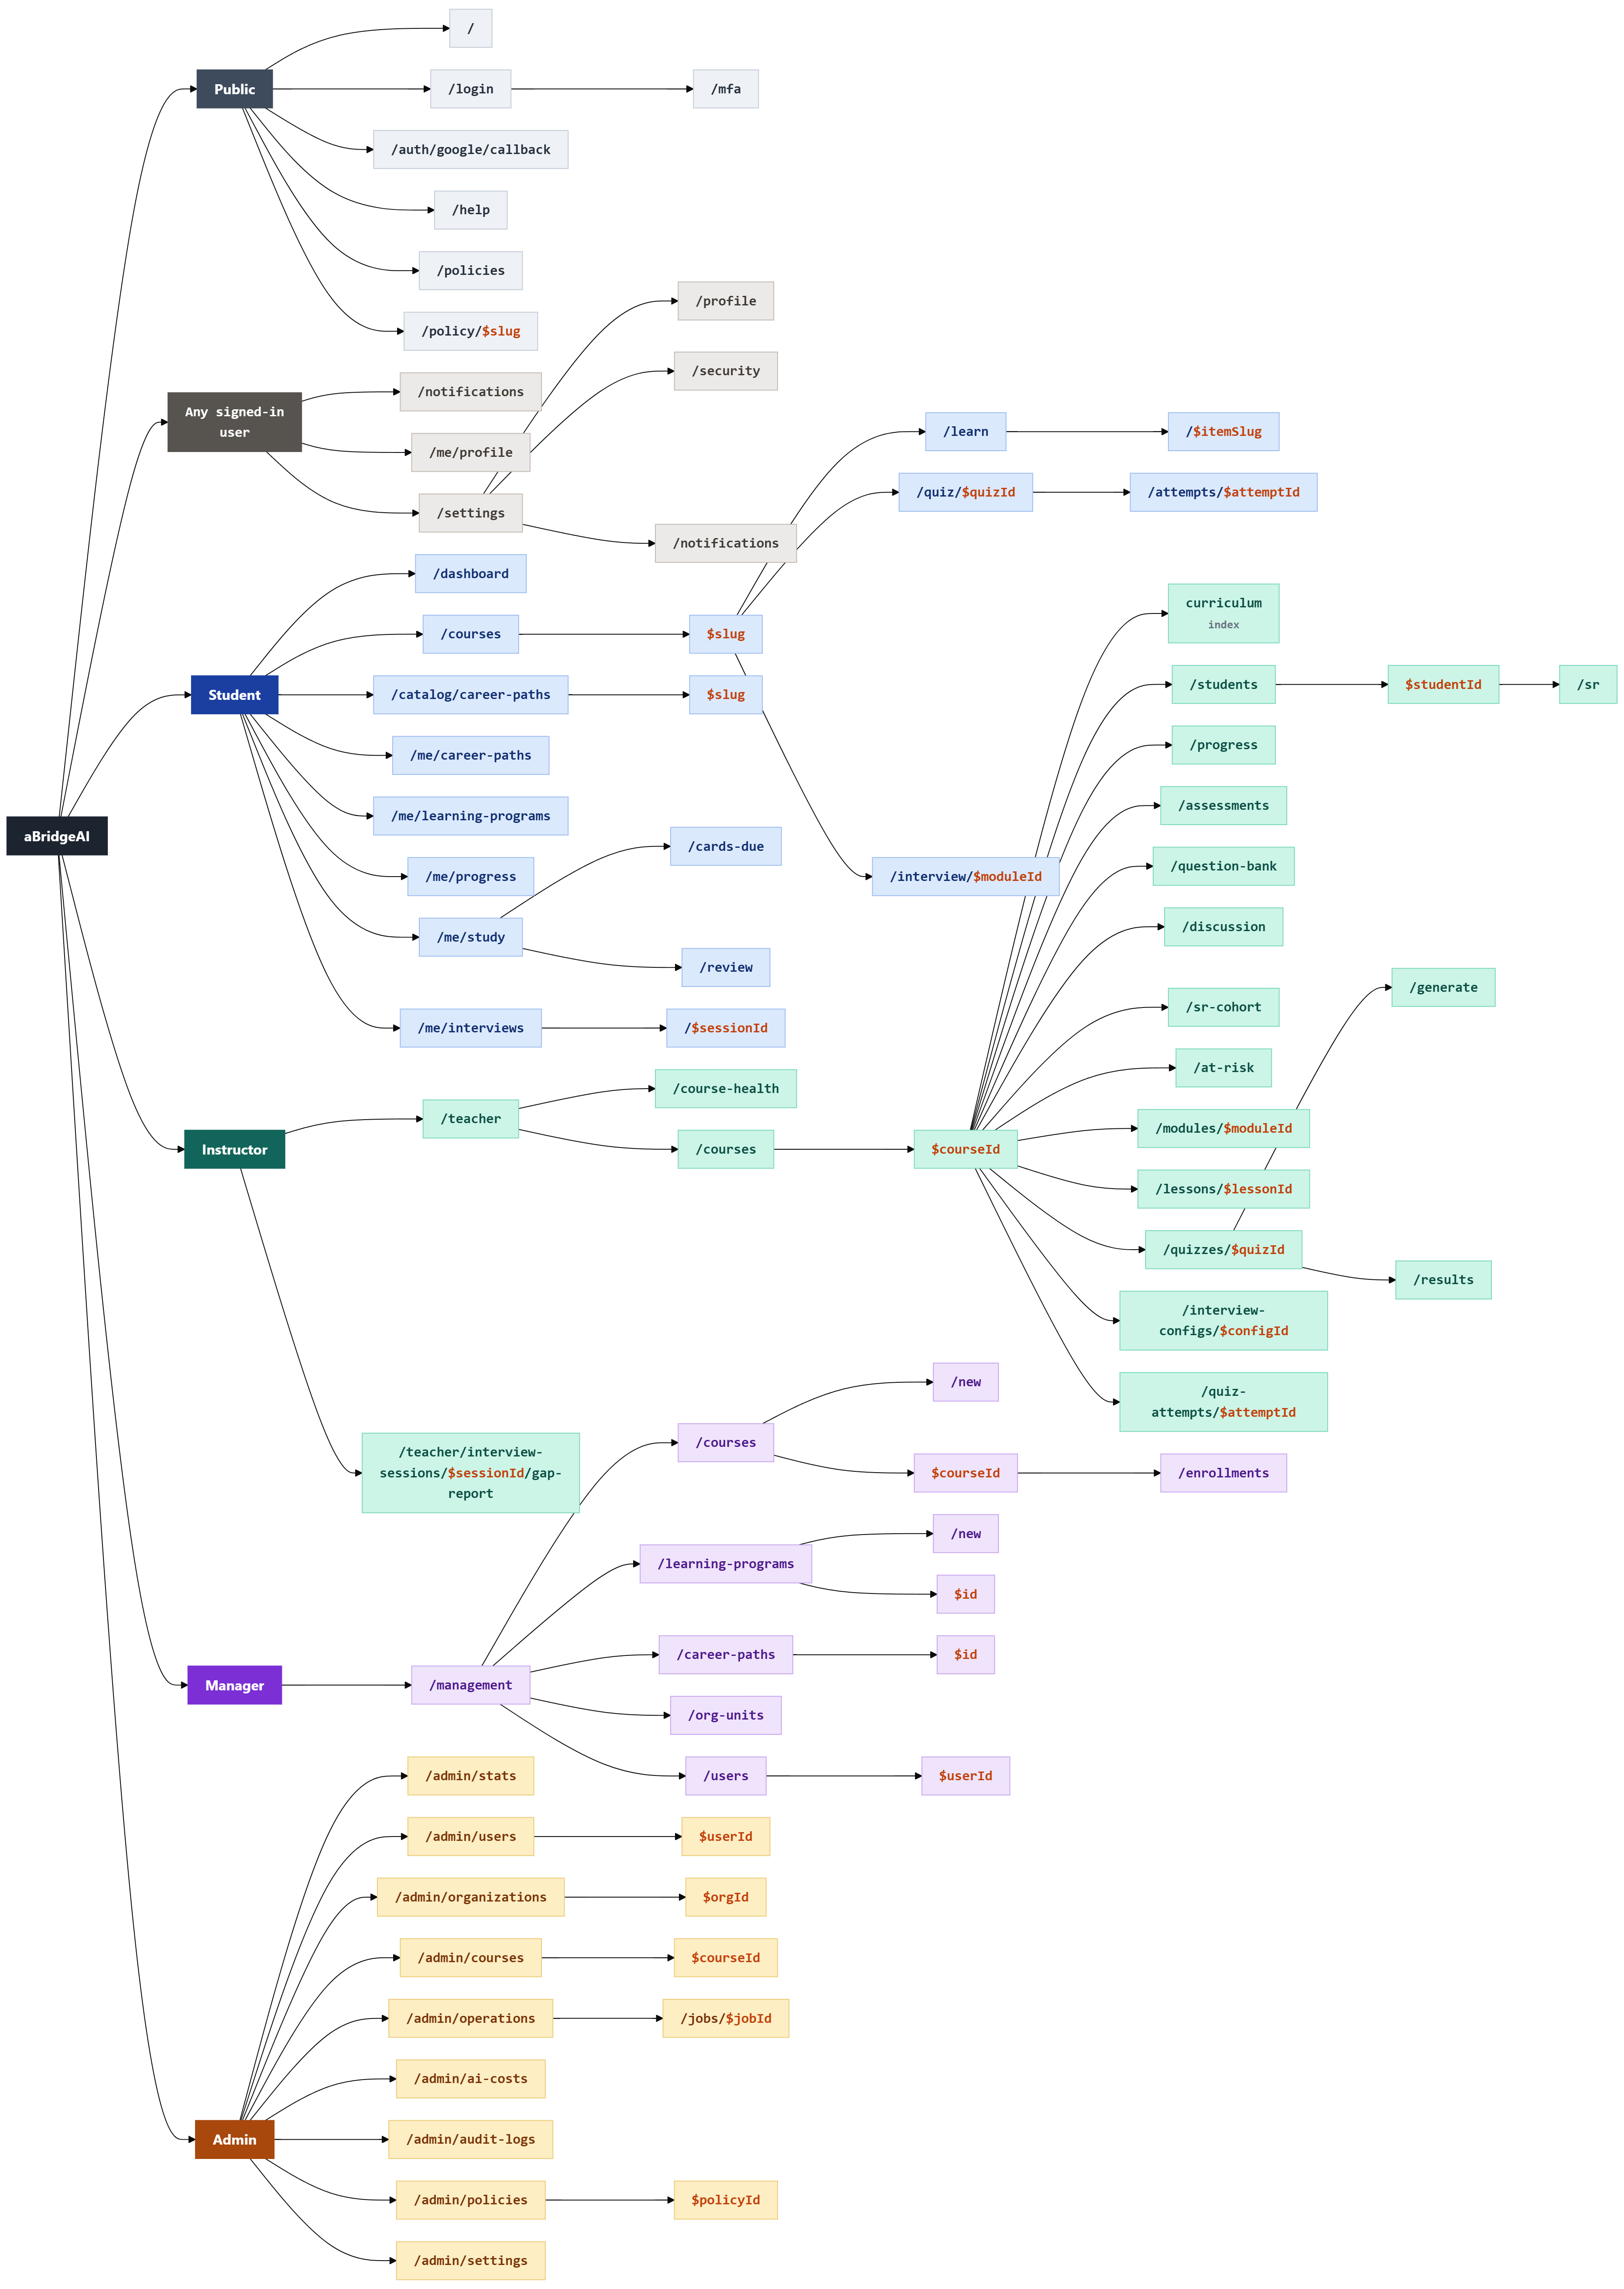
\includegraphics[width=\textwidth,height=0.85\textheight,keepaspectratio]{graphics/screenshots/sitemap_diagram.png}
    \caption{Application sitemap --- colour-coded by band: cool grey (public), warm grey (any signed-in user), blue (student), teal (instructor), violet (educational manager), amber (administrator). Dynamic URL segments are highlighted in amber as \texttt{\$param}. Every node is one destination route; the 16 redirect-only aliases are omitted here and listed in Table~\ref{tab:sitemap_redirects}.}
    \label{fig:sitemap}
\end{figure}

The sitemap is intentionally flat within each role group: there are no role-specific subdomains, only path prefixes, so a single deployment serves every persona. Three prefixes are privileged --- \path|/admin|, \path|/teacher| and \path|/management| --- and each maps to exactly one permission set, so the section a URL belongs to and the permission it demands are the same fact written once. A band names the persona a route is designed for, not the permission it demands, and the two are deliberately not the same partition. The notification inbox, the account settings pages, and the reader's own profile hang off the top bar, which the application shell renders for every authenticated role, so they belong to no single persona and are drawn in a band of their own. The remaining learner routes are equally ungated --- a teacher who types \path|/me/study| reaches it --- and sit under \textit{Student} only because that is the sidebar which offers them. The learner surfaces carry two unprivileged prefixes of their own: \path|/me| for everything scoped to the signed-in user, and \path|/catalog| for the organisation-wide browsable inventory, which keeps \emph{my} career paths distinct from \emph{the} career paths. Role differentiation is enforced by the \path|beforeLoad| guard on the parent route, a prefix-to-permission check in the authenticated layout, and the role-specific navigation groups driving the sidebar. This keeps the bundle small (one client-side router for the whole platform) and makes it cheap to add new role-scoped routes --- a new admin page is one new \path|createRoute| call that joins the \path|authenticatedRoute| children list.
